\section{Results}
When examining the presence of various game engines on Steam for 2018, 2022, and 2023, it is important to see the significance of these results in the context of indie game development.
The following \autoref{table:steam} presents the percentages of game engines on Steam for these years.

\begin{table}[ht!]
    \centering
    \begin{tabular}{|c c c c|}
        \hline
        Game Engine & 2018   & 2022    & 2023    \\
        \hline\hline
        Unity       & 25.6\% & 61.22\% & $\textcolor{red}{\blacktriangledown 60.04\%}$  \\
        Unreal      & 13.2\% & 15.91\% & $\textcolor{ForestGreen}{\blacktriangleup 16.42\%}$  \\
        Source      & 4.0\%  & 0.27\%  & $\textcolor{red}{\blacktriangledown 0.23\%}$   \\
        CryEngine   & 3.5\%  & 0.23\%  & $\textcolor{red}{\blacktriangledown 0.19\%}$   \\
        GameBryo    & 3.2\%  & -       & -       \\
        IW          & 2.9\%  & -       & -       \\
        Anvil       & 2.5\%  & 0.05\%  & $\textcolor{gray}{\bullet 0.05\%}$   \\
        id Tech     & 1.7\%  & 0.18\%  & $\textcolor{red}{\blacktriangledown 0.15\%}$   \\
        Essence     & 1.1\%  & -       & -       \\
        Clausewitz  & 1.0\%  & 0.03\%  & $\textcolor{red}{\blacktriangledown 0.02\% }$  \\
        Other       & 48.4\% & 22.17\% & $\textcolor{ForestGreen}{\blacktriangleup 22.94\%}$  \\
        \hline
    \end{tabular}
    \caption{Percentage of total games identified on Steam (data collected 2022-09-30 and 2023-10-21)}
    \label{table:steam}
\end{table}

Game engines that have experienced an increase in their percentage of total games developed in comparison to the previous year(s) are highlighted in green, indicating a positive trend, while those that have seen a decrease are highlighted in red, suggesting a decline in their usage over the same period.
The data from 2018 was collected using the Wikipedia method, while the data from 2022 and 2023 was collected using the pattern matching method. 
Color-coding in \autoref{table:steam} is missing for the column for 2022. 
This is due to the differing data collection methods used in 2018.
It is difficult to say whether the newer method can attribute more game engines or simply more games were created using a particular game engine.
To illustrate, consider Unity, which has 35.62\% more share of all identified games from 2018 to 2022.
Additionally, it is worth noting that among the game engines analyzed, only the Unreal Engine has consistently exhibited growth over the various years.
This trend holds true when considering both the complete dataset, which includes 2018 data, and the dataset from 2022 and 2023 alone. 
The Godot Engine is not listed in \autoref{table:steam} because the paper from Toftedahl and Engström did not include it in their analysis.
Despite this omission, the data remains valuable in shedding light on changing market dynamics. \\

Between 2022 and 2023, it is noteworthy that other game engines have also gained increased popularity, indicating shifts in the competitive landscape.
At the time of the collected data in 2022, 1.15\% of all games created with the Godot Engine were identified.
However, in 2023, this percentage increased to 1.44\%.
Compared to the other game engines on SteamDB, the Godot Engine ranks 6th out of 65 recognized game engines.
In addition to that it is important to understand that the percentages from \autoref{table:steam} represent lower bounds.
Particularly in the case of the Godot engine, there could be a lot more games.
This is due to the fact that the Godot Engine allows for the export of executables without a recognizable filename signature, making them unidentifiable by the SteamDB algorithm.
Consequently, only a subset of games with specific filename patterns can be matched. \\
% Refactor(discussion): This ranking suggests a noteworthy level of relevance in the video game industry for the Godot Engine, given its relatively high position among recognized game engines.

\begin{figure}[ht!]
    \begin{center}
        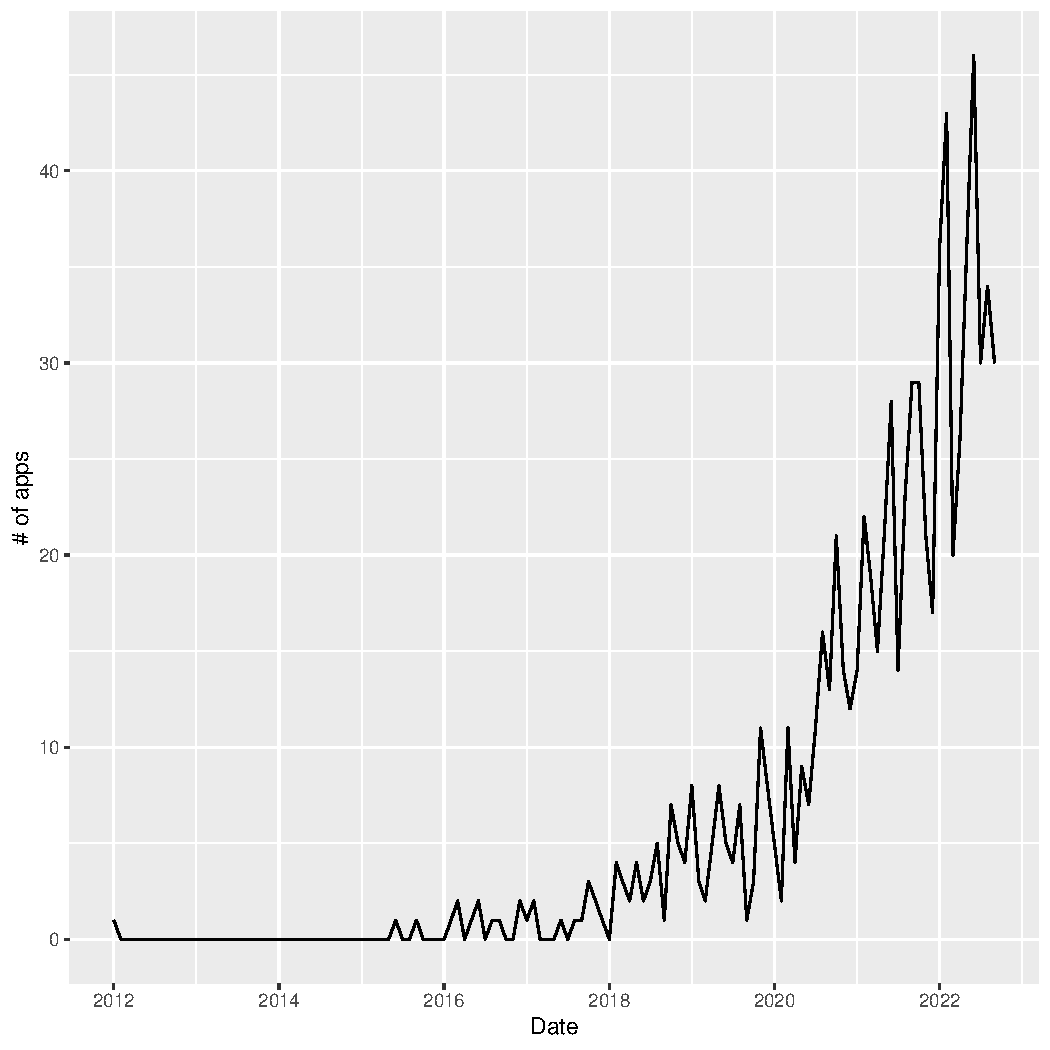
\includegraphics[width=1\columnwidth]{figures/godot-graph.pdf}
        \caption{\label{fig:godot-graph} Number of released Apps on Steam per month}
    \end{center}
\end{figure}

An examination of the monthly app releases depicted in \autoref{fig:godot-graph}, a clear trend emerges: in 2020, there was a significant increase in the number of released games.
This increase in game releases prompts further investigation to understand the underlying reasons.
Prior to conducting a more in-depth analysis of the underlying reasons, we first draw a parallel by comparing the data from itch.io.
In contrast to Steam, the digital sales platform itch.io predominantly showcases indie games, aligning with the specific focus of this paper.
Unlike Steam, itch.io possesses an official statistics website that provides information on game engines \cite{itchio-engines}.
However, it's essential to acknowledge that this data might be incomplete due to its reliance on self-reporting.
Therefore, there may be gaps or inaccuracies in the information, a limitation inherent to self-reported data. \\

\begin{table}[ht!]
    \centering
    \begin{tabular}{|c c c c|}
        \hline
        Game Engine & 2018   & 2022                                                & 2023                                                \\
        \hline\hline
        Unity       & 47.3\% & $\textcolor{ForestGreen}{\blacktriangleup 49.75\%}$ & $\textcolor{red}{\blacktriangledown 46.33\%}$       \\
        Construct   & 12.3\% & $\textcolor{ForestGreen}{\blacktriangleup 13.12\%}$ & $\textcolor{ForestGreen}{\blacktriangleup 13.82\%}$ \\
        GameMaker   & 11.0\% & $\textcolor{red}{\blacktriangledown 7.32\%}$        & $\textcolor{red}{\blacktriangledown 6.95\%}$        \\
        Twine       & 6.2\%  & $\textcolor{red}{\blacktriangledown 5.35\%}$        & $\textcolor{ForestGreen}{\blacktriangleup 6.03\%}$  \\
        RPG Maker   & 3.9\%  & $\textcolor{red}{\blacktriangledown 2.74\%}$        & $\textcolor{ForestGreen}{\blacktriangleup 2.76\%}$  \\
        Bitsy       & 3.3\%  & $\textcolor{red}{\blacktriangledown 3.11\%}$        & $\textcolor{ForestGreen}{\blacktriangleup 3.18\%}$  \\
        PICO-8      & 2.9\%  & $\textcolor{red}{\blacktriangledown 2.68\%}$        & $\textcolor{red}{\blacktriangledown 2.60\%}$        \\
        Unreal      & 2.8\%  & $\textcolor{ForestGreen}{\blacktriangleup 2.92\%}$  & $\textcolor{ForestGreen}{\blacktriangleup 3.01\%}$  \\
        Godot       & 2.5\%  & $\textcolor{ForestGreen}{\blacktriangleup 5.55\%}$  & $\textcolor{ForestGreen}{\blacktriangleup 7.51\%}$  \\
        Ren'Py      & 2.0\%  & $\textcolor{red}{\blacktriangledown 1.93\%}$        & $\textcolor{ForestGreen}{\blacktriangleup 2.07\%}$  \\
        Other       & 5.9\%  & $\textcolor{red}{\blacktriangledown 5.55\%}$        & $\textcolor{ForestGreen}{\blacktriangleup 5.75\%}$  \\
        \hline
    \end{tabular}
    \caption{Percentage of total games identified on itch.io (data collected 2022-09-30 and 2023-10-21)}
    \label{table:itch}
\end{table}

Similar to Steam, the data from itch.io can be compared to the 2018 reference paper using the most current data available from 2022 and 2023.
The consistent data collection method allows for direct comparisons, as illustrated in \autoref{table:itch}.
Upon comparing the data presented in \autoref{table:steam} and \autoref{table:itch}, Unity stands out as a prevalent game engine.
In both 2022 and 2023, Unity consistently constitutes over half of all games on Steam and nearly half on itch.io.
This dominance is particularly striking when considering the second-ranking game engines, which represent approximately 16\% of games on Steam and roughly 14\% on itch.io in 2023.
A similar trend can be observed for 2022. \\

It can also be seen that besides Unity only three other game engines have consistently gained popularity on itch.io.
These three game engines are Construct, Unreal and Godot Engine.
Construct is a game engine primarily aimed at non-programmers.
With the help of visual programming, it is intended to make it easier for novice programmers to get started.
The notable increase in its percentage of games may be attributed to the appeal of game development to a broader audience with limited coding expertise.
However, this is only an assumption that needs to be investigated further. \\

While the Unreal Engine prominently appears as the second most used game engine on Steam, its presence on itch.io has seen only marginal growth over the past four to five years.
This is particularly interesting as it suggests that the Unreal Engine holds a limited relevance among indie game developers.
% refactor(discussion) The Unreal Engine is often referred to as the game engine for AAA games \cite{unreal-tripple-a-yager, unreal-tripple-a-india}.
% refactor(discussion) This could be one of the reasons why indie game developers have less interest in this game engine. \\

Looking at \autoref{table:itch}, it is evident that the Godot Engine has experienced remarkable growth in popularity on itch.io.
To delve deeper into this trend, a dedicated script was developed to compile games from itch.io along with their release dates, resulting in a CSV file \cite{github-trend-itch}.
It should be mentioned that not all games could be fetched with this script.
Despite the missing data sets of up to about 10\% of the games, it is still possible to create a trend plot for the game engines listed in \autoref{table:itch}.

\begin{figure}[ht!]
    \begin{center}
        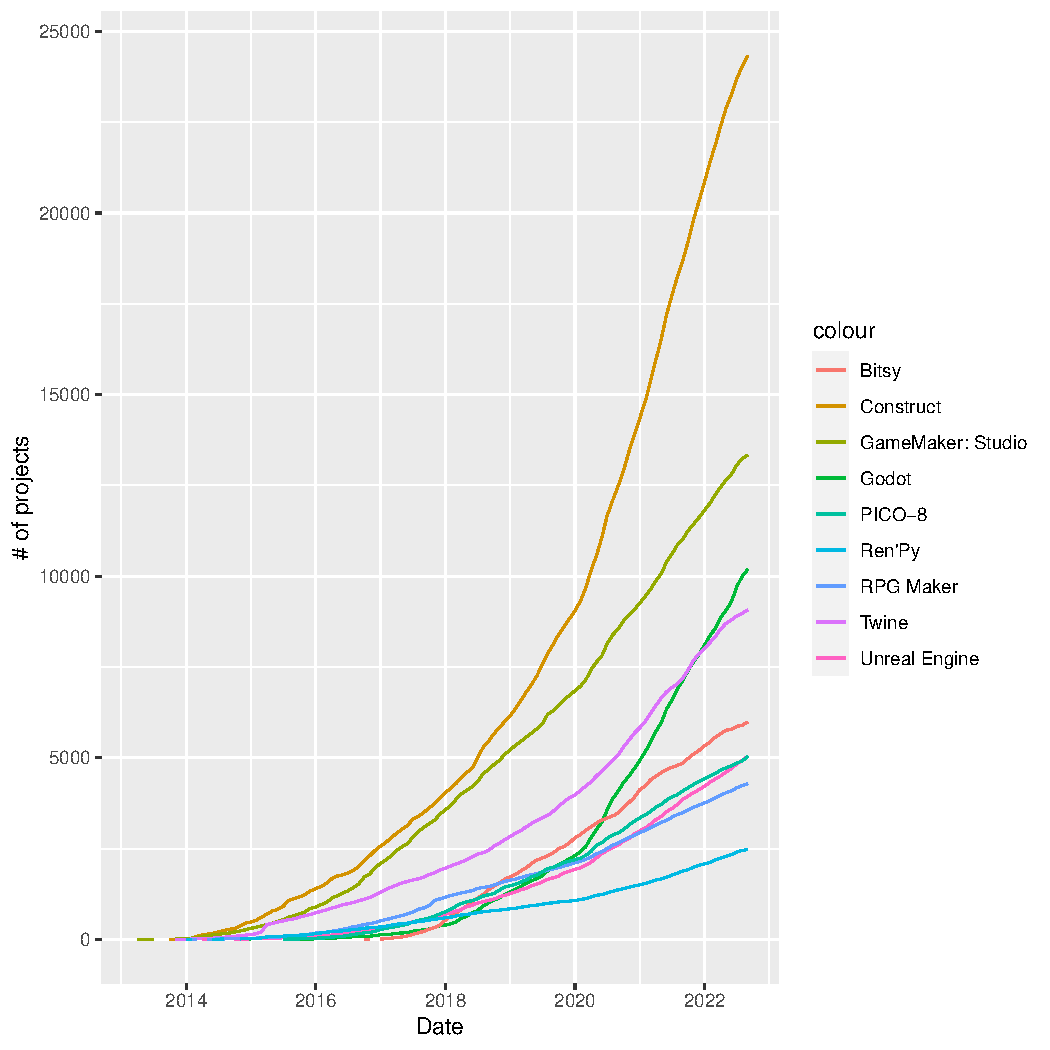
\includegraphics[width=1.1\columnwidth]{figures/trend-graph.pdf}
        \caption{\label{fig:trend-graph} Cumulative sum of the number of projects on itch.io}
    \end{center}
\end{figure}

This graph is shown in \autoref{fig:trend-graph}.
Notably, Unity, due to its large number of projects, has been excluded from the graph to ensure better visibility and clarity for the other game engines.
It is evident that the Godot Engine has gained a significant surge in popularity in 2020, surpassing both Bitsy and Twine.
% refactor(discussion) However, pinpointing the exact reasons for the Godot Engine's remarkable growth from the beginning of 2020 is challenging due to the multitude of potential factors involved.
% refactor(discussion) Likewise, important events may have taken place before 2020 that just took longer to become noticeable.
% refactor(discussion) Therefore, only assumptions can be made about the growth in popularity.
This analysis has its limitations, as it relies on the quantity of games published.
It does not consider factors like the quality or number of games published by individual publishers.
Determining the percentage of actual indie game studios is also challenging, because not every publisher was analyzed individually.

\begin{table}[ht!]
    \centering
    \begin{tabular}{|c c c c c|}
        \hline
        Game Engine & 2020   & 2021                                               & 2022                                               & 2023                                             \\
        \hline\hline
        Unity       & 62.2\% & $\textcolor{red}{\blacktriangledown 61.6\%}$       & $\textcolor{red}{\blacktriangledown 61.1\%}$       & $\textcolor{red}{\blacktriangledown 59\%}$       \\
        Godot       & 12.2\% & $\textcolor{ForestGreen}{\blacktriangleup 13.1\%}$ & $\textcolor{ForestGreen}{\blacktriangleup 15.6\%}$ & $\textcolor{ForestGreen}{\blacktriangleup 19\%}$ \\
        GameMaker   & 10.9\% & $\textcolor{red}{\blacktriangledown 8.9\% }$       & $\textcolor{red}{\blacktriangledown 6.1\%}$        & $\textcolor{red}{\blacktriangledown 5\%}$        \\
        Unreal      & -      & 4.2\%                                              & $\textcolor{ForestGreen}{\blacktriangleup 4.8\%}$  & -                                                \\
        Construct   & 1.7\%  & $\textcolor{ForestGreen}{\blacktriangleup 2.4\%}$  & $\textcolor{red}{\blacktriangledown 1.7\%}$        & -                                                \\
        Stencyl     & 0.1\%  & 0.1\%                                              & -                                                  & -                                                \\
        Other       & 12.9\% & $\textcolor{red}{\blacktriangledown 6.5\%}$        & $\textcolor{ForestGreen}{\blacktriangleup 7.0\%}$  & $\textcolor{ForestGreen}{\blacktriangleup 17\%}$ \\
        No engine   & -      & 3.1\%                                              & $\textcolor{ForestGreen}{\blacktriangleup 3.7\%}$  & -                                                \\
        \hline
    \end{tabular}
    \caption{Used game engines by GMTK Game Jam participants over the years \cite{gmtk-twitter}}
    \label{table:gmtk}
\end{table}

An interesting distinction on itch.io, which is not as prominent on Steam, is the prevalence of games created during game jams, which are defined as follows:
\blockquote{A game jam is an accelerated opportunistic game creation event where a game is created in a relatively short timeframe exploring given design constraint(s) and end results are shared publically \cite{game-jam-definition}.}
With around 18,000 - 23,000 participants and around 6,000 - 7,000 submissions, GMTK Game Jam is the largest past game jam event on itch.io \cite{gmtk-game-jam-2021, gmtk-game-jam-2022, gmtk-game-jam-2023}.
\autoref{table:gmtk} shows the game engines used by participants in the events from 2020 to 2023.
This table is clearly showing that the Godot Engine is the only game engine from the table to outperform the usage of the previous year three years in a row. \\
% refactor(discussion) This observation raises the possibility that game jams on itch.io may contribute to the sustained relevance of the Godot Engine.
% refactor(discussion) It is important to consider that the overall popularity of a game engine could lead to its increased utilization in game jams. \\

% refactor(discussion) To make more accurate assessments, it is essential to compare the Godot Engine with other game engines that have gained popularity on itch.io.
% refactor(discussion) The Godot Engine can be categorized as a general-purpose game engine, covering a wide range of game genres.
% refactor(discussion) According to Toftedahl and Engström, this puts it in the same category as the Unreal Engine and Unity.
% refactor(discussion) Construct, on the other hand, is a special purpose game engine.
% refactor(discussion) In the introduction, it was already explained that game engines should be compared with each other in terms of a specific purpose.
% refactor(discussion) For this reason, Construct should not be included in a comparison.
% refactor(discussion) A meaningful comparison would require a feature matrix, benchmarks, or other technical aspects, which is beyond the scope of this paper and warrants a separate investigation.
% refactor(discussion) In this paper, the focus is specifically on the Godot Engine and its significance within the indie game industry.
% refactor(discussion) However, this work can provide the basis for which game engines should be compared with each in the context of the indie game industry.\\

% TODO: analyze Poll 2023
To explore more about the Godot Engine, the Godot Community Poll from 2022 was examined \cite{godot-poll-results}.
This survey contains 5315 answers to a variety of questions.
When asked about previous experience with other game engines, the top three were Unity (51\%), Other third party engine (30.6\%), and GameMaker (22\%).
With Unity having a strong presence on both Steam and itch.io, it seems natural that developers would have been in contact with the game engine in advance.
It is difficult to make a correct statement about other third party engines due to the lack of specificity.
However, a statement, or rather an assumption, can be made about GameMaker.
If you take a closer look at \autoref{table:gmtk}, it becomes clear that GameMaker is the only game engine that has lost an extremely large percentage of its users.
It could therefore be possible that these developers have switched from GameMaker to the Godot Engine.\\

If we look at the data for the usage of the Godot Engine in the poll, we can see that 56.56\% of the respondents primarily use the Godot Engine for 2D game development.
This is in contrast to the usage of 35.22\% in 3D game development.
It can be said that the Godot Engine has the possibility to develop 2D, 3D and especially XR, but it is primarily used for 2D. \\
% refactor(discussion) Several factors could contribute to this trend.
% refactor(discussion) On one hand, the Godot Engine could provide more robust functionality for 2D game development compared to its 3D capabilities. 
% refactor(discussion) Additionally, the workload associated with 3D game development is typically higher than that of 2D, which may pose challenges for indie game developers, leading them to favor 2D development.\\

The survey's focus on indie game developers becomes evident when examining the respondents profiles.
A substantial 84\% of participants stated that they use the Godot Engine as a hobby, while 9\% identified themselves as full-time indie game developers. 
According to the definition outlined in this paper, hobby developers fall under the category of indie game developers, as they share common characteristics such as focusing on specific goals, lacking financial support from larger companies, and working in small teams. 
This is further supported by the finding that 97.9\% work on their project alone or in a team of up to five people.
Furthermore, the survey reveals that 83.7\% of respondents do not earn any income from their games, emphasizing their indie status.
Additionally, the two most prevalent digital sales platforms among respondents are itch.io (7.1\%) and Steam (6\%). \\
% refactor(discussion) The higher representation of itch.io over Steam in the survey data may suggest that the Godot Engine holds greater relevance for indie game developers. 

The survey data provides insights into the increasing relevance of the Godot Engine in 2020
The majority of respondents (22.2\%) had already learned about the Godot Engine in 2019.
However, most of them (21.9\%) started using the engine for programming in the following year, 2020.
% refactor(discussion) This finding supports the statement that there may have been important events before 2020 that took longer to convince people to develop.
% refactor(discussion) A hypothetical scenario could involve an indie game developer who shared their progress with the Godot Engine through individual YouTube videos.
% refactor(discussion) These videos may have drawn attention to the Godot Engine in 2019.
% refactor(discussion) As interest in the engine grew, the developer may have decided to publish tutorials in 2020, motivating many individuals to begin development with the Godot Engine.
% refactor(discussion) It's essential to note that this scenario is just one possibility among many, and the actual reasons for the increase in Godot Engine usage in 2020 are likely diverse.
